\label{sec:formalize}
\subsection{Khái niệm}
Học tăng cường (thuật ngữ gốc: \emph{Reinforcement Learning-RL})\cite{sutton1998introduction} là một trong ba kiểu học máy chính bên cạnh học giám sát (thuật ngữ gốc: \emph{Supervised Learning}) và học không giám sát (thuật ngữ gốc: \emph{Unsupervised Learning}). Bản chất của RL là thử và sai (thuật ngữ gốc: \emph{trial-and-error}, nghĩa là thử đi thử lại và rút ra kinh nghiệm sau mỗi lần thử như vậy. Tương tự như các hệ thống trí tuệ nhân tạo khác, một hệ thống RL bao gồm tác nhân (thuật ngữ gốc: \emph{agent}) và môi trường (thuật ngữ gốc: \emph{environment}). Agent là bất cứ những thứ gì có thể cảm nhận\cite{russell2009artificial} được từ môi trường của nó thông qua các cảm biến và tác động của môi trường. 
Environment là một vấn đề, một bài toán mà agent phải giải quyết. Thêm vào đó trong hệ thống RL có thêm 3 thành phần chính: chính sách (thuật ngữ gốc: \emph{policy}), phần thưởng (thuật ngữ gốc: \emph{reward}), hàm giá trị (thuật ngữ gốc: \emph{value fucntion}). Nói một cách ngắn gọn mục tiêu của một hệ thống RL đó là cố gắng để học policy nhận được về từ environment bằng cách sử dụng các giá trị reward thu được sao cho tổng reward thu được là lớn nhất. Trước tiên ta cùng thống nhất một số định nghĩa như sau:
\begin{itemize}
    \item \emph{policy} là một ánh xạ từ các trạng thái
của môi trường đến một hành động phù hợp trong trạng thái đó. Nó có thể như là một bảng tra cứu đơn giản, một quy tắc hay một quá trình tính toán phức tạp. 
    \item \emph{reward} là mục tiêu cần đạt được trong RL. Tại mỗi thời điểm, environment sẽ gửi về agent một giá trị vô hướng gọi là reward. Mục đích của tổng reward thi được trong thời gian lâu dài. Giá trị reward thu được sẽ tương ứng với việc hành động tác động đến môi trường là tốt hay xấu.
    \item \emph{value function} biểu thị mức độ tốt của trạng thái hiện tại của môi trường đối với agent. Nó tương đương với tổng reward dự kiến mà agent có thể nhận được tại các trạng thái tiếp theo kể từ hiện tại.
\end{itemize}
Người học trong RL được gọi là agent phải học để có thể tìm được hành động phù hợp với trạng thái của môi trường sao cho tối đa hóa tổng reward thu được. Agent phải khám phá ra chuỗi những hành động nào đem lại tổng reward cho nó.

\subsection{Chu trình Markov trong RL}
\begin{figure}[ht]
    \centering
    \fbox{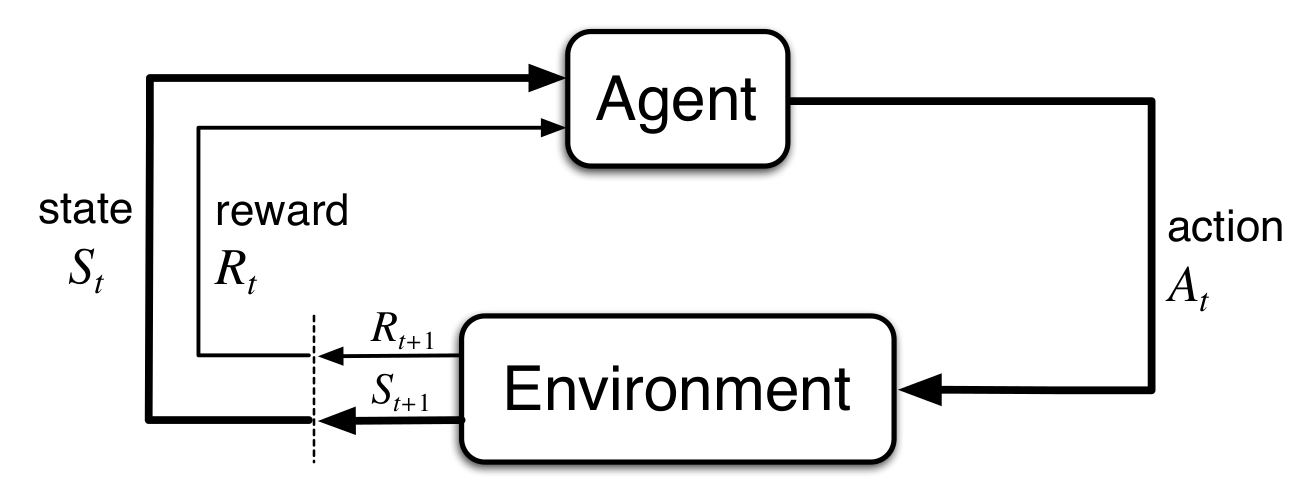
\includegraphics[width=0.65\linewidth]{images/mdp.png}}
    \caption{Chu trình học trong học tăng cường}
    \label{fig:problem:mdp}
\end{figure}
Toàn bộ quá trình, mục đích RL ở trên có thể mô tả bằng cách sử dụng ý tưởng của \emph{Markov Decision Process - MDP} cho các hệ thống động. MDP là một khung đơn giản cho việc học hỏi từ sự tương tác để đạt được một mục tiêu. Agent và environment tương tác liên tục, agent chọn hành động và environment phản ứng với những hành động này và đưa ra các tình huống mới cho agent. 

Trong hệ thống RL agent và environment sẽ tương tác với nhau tại các thời điểm $t=0,1,2,3...$. Tại mỗi thời điểm $t$, agent sẽ nhận được một mô tả trạng thái hiện tại của môi trường $S_t \in \delta$. Tại thời điểm kế tiếp agent sẽ nhận được một giá trị $reward$ tương ứng với hành động $A_{t}$ trước đó của nó là reward $R_{t+1} \in \mathcal{R} \subset \mathbb{R}$ và đưa nó đến trạng thái mới là $S_{t+1}$. Cứ như vậy agent và environment cùng tạo ra một vòng lặp: $S_{0}, A_{0}, R_{1}, S_{1}, A_{1}, R_{2}, S_{2}, A_{2}, R_{3}, \dots$. Việc biểu diễn này rất quan trọng, khi mà ta không phải lưu một chuỗi các states trước đó để biểu diễn state hiện tại khiến cho việc tính toán trở nên phức tạp và tiêu tốn bộ nhớ.
Sau chu trình này, agent sẽ đạt được tổng số reward tương đương với giá trị tối đa của value function:
\begin{equation}
    G_{t} \doteq R_{t+1}+R_{t+2}+R_{t+3}+\cdots+R_{T}
\end{equation}
Giá trị tối đa này chính là tổng reward lớn nhất mà agent có thể nhận được sau một thời gian lâu dài. 
